% This is "sig-alternate.tex" V2.0 May 2012
% This file should be compiled with V2.5 of "sig-alternate.cls" May 2012
%
% This example file demonstrates the use of the 'sig-alternate.cls'
% V2.5 LaTeX2e document class file. It is for those submitting
% articles to ACM Conference Proceedings WHO DO NOT WISH TO
% STRICTLY ADHERE TO THE SIGS (PUBS-BOARD-ENDORSED) STYLE.
% The 'sig-alternate.cls' file will produce a similar-looking,
% albeit, 'tighter' paper resulting in, invariably, fewer pages.
%
% ----------------------------------------------------------------------------------------------------------------
% This .tex file (and associated .cls V2.5) produces:
%       1) The Permission Statement
%       2) The Conference (location) Info information
%       3) The Copyright Line with ACM data
%       4) NO page numbers
%
% as against the acm_proc_article-sp.cls file which
% DOES NOT produce 1) thru' 3) above.
%
% Using 'sig-alternate.cls' you have control, however, from within
% the source .tex file, over both the CopyrightYear
% (defaulted to 200X) and the ACM Copyright Data
% (defaulted to X-XXXXX-XX-X/XX/XX).
% e.g.
% \CopyrightYear{2007} will cause 2007 to appear in the copyright line.
% \crdata{0-12345-67-8/90/12} will cause 0-12345-67-8/90/12 to appear in the copyright line.
%
% ---------------------------------------------------------------------------------------------------------------
% This .tex source is an example which *does* use
% the .bib file (from which the .bbl file % is produced).
% REMEMBER HOWEVER: After having produced the .bbl file,
% and prior to final submission, you *NEED* to 'insert'
% your .bbl file into your source .tex file so as to provide
% ONE 'self-contained' source file.
%
% ================= IF YOU HAVE QUESTIONS =======================
% Questions regarding the SIGS styles, SIGS policies and
% procedures, Conferences etc. should be sent to
% Adrienne Griscti (griscti@acm.org)
%
% Technical questions _only_ to
% Gerald Murray (murray@hq.acm.org)
% ===============================================================
%
% For tracking purposes - this is V2.0 - May 2012

\documentclass{sig-alternate}
\usepackage[latin1]{inputenc}
\usepackage{graphicx}        % standard LaTeX graphics tool
\usepackage{subfigure}
\usepackage{url}


\begin{document}
%
% --- Author Metadata here ---
\conferenceinfo{GECCO'14,} {July 12-16, 2014, Vancouver, BC, Canada.}
    \CopyrightYear{2014}
    \crdata{TBA}
    \clubpenalty=10000
    \widowpenalty = 10000

\title{Fighting to Survive: Evolving RTS Bots without Evaluation}

\subtitle{[Abstract]}
%\titlenote{A full version of this paper is available as
%\textit{Author's Guide to Preparing ACM SIG Proceedings Using
%\LaTeX$2_\epsilon$\ and BibTeX} at
%\texttt{www.acm.org/eaddress.htm}}}
%
% You need the command \numberofauthors to handle the 'placement
% and alignment' of the authors beneath the title.
%
% For aesthetic reasons, we recommend 'three authors at a time'
% i.e. three 'name/affiliation blocks' be placed beneath the title.
%
% NOTE: You are NOT restricted in how many 'rows' of
% "name/affiliations" may appear. We just ask that you restrict
% the number of 'columns' to three.
%
% Because of the available 'opening page real-estate'
% we ask you to refrain from putting more than six authors
% (two rows with three columns) beneath the article title.
% More than six makes the first-page appear very cluttered indeed.
%
% Use the \alignauthor commands to handle the names
% and affiliations for an 'aesthetic maximum' of six authors.
% Add names, affiliations, addresses for
% the seventh etc. author(s) as the argument for the
% \additionalauthors command.
% These 'additional authors' will be output/set for you
% without further effort on your part as the last section in
% the body of your article BEFORE References or any Appendices.


\numberofauthors{2}
 \author{
 \alignauthor
 Bot1\\
        \affaddr{BotLand Institute of Techonology (BIT)}\\
        \affaddr{CPU Street num. 1110010}\\
        \affaddr{BotLand}\\
        \email{bot1@bit.com}
 \alignauthor
 Bot2\\
 \affaddr{Bots University (BU)}\\
 \affaddr{ALU Street num. 101110}\\
 \affaddr{Metropolis}\\
 \email{bot2@bu.com}
 }

%\numberofauthors{2}
% \author{
% \alignauthor
% J.J. Merelo, A.M. Mora, C. M. Fernandes\\
%        \affaddr{University of Granada}\\
%        \affaddr{Department of Computer Architecture and Technology, ETSIIT}\\
%        \affaddr{18071 - Granada}\\
%        \email{jmerelo,amorag,cfernandes@geneura.ugr.es}
% \alignauthor
% Anna I. Esparcia-Alc�zar\\
% \affaddr{S2 Grupo}\\
% \email{aesparcia@s2grupo.es}
% }


%\numberofauthors{4} %  in this sample file, there are a *total*
% of EIGHT authors. SIX appear on the 'first-page' (for formatting
% reasons) and the remaining two appear in the \additionalauthors section.
%

%\author{
% You can go ahead and credit any number of authors here,
% e.g. one 'row of three' or two rows (consisting of one row of three
% and a second row of one, two or three).
%
% The command \alignauthor (no curly braces needed) should
% precede each author name, affiliation/snail-mail address and
% e-mail address. Additionally, tag each line of
% affiliation/address with \affaddr, and tag the
% e-mail address with \email.
%
% 1st. author
%\alignauthor
%Jack\\
%       \affaddr{Lost island}\\
%       \affaddr{unknow}\\
%       \affaddr{Pacific Ocean}\\
%       \email{jack_the_doctor@lost.com}
% 2nd. author
%\alignauthor
%Sawyer\\
%       \affaddr{Lost island}\\
%       \affaddr{unknow}\\
%       \affaddr{Pacific Ocean}\\
%       \email{sawyer_tom@lost.com}
% 3rd. author
%\alignauthor 
%Lock\\
%       \affaddr{Lost island}\\
%       \affaddr{unknow}\\
%       \affaddr{Pacific Ocean}\\
%       \email{lock@lost.com}
% 4rd. author
%\alignauthor 
%Hurley\\
%       \affaddr{Lost island}\\
%       \affaddr{unknow}\\
%       \affaddr{Pacific Ocean}\\
%       \email{hugo@lost.com}
%}

%\and  % use '\and' if you need 'another row' of author names
% 4th. author
%\alignauthor Lawrence P. Leipuner\\
%       \affaddr{Brookhaven Laboratories}\\
%       \affaddr{Brookhaven National Lab}\\
%       \affaddr{P.O. Box 5000}\\
%       \email{lleipuner@researchlabs.org}
% 5th. author
%\alignauthor Sean Fogarty\\
%       \affaddr{NASA Ames Research Center}\\
%       \affaddr{Moffett Field}\\
%       \affaddr{California 94035}\\
%       \email{fogartys@amesres.org}
% 6th. author
%\alignauthor Charles Palmer\\
%       \affaddr{Palmer Research Laboratories}\\
%       \affaddr{8600 Datapoint Drive}\\
%       \affaddr{San Antonio, Texas 78229}\\
%       \email{cpalmer@prl.com}
%}
% There's nothing stopping you putting the seventh, eighth, etc.
% author on the opening page (as the 'third row') but we ask,
% for aesthetic reasons that you place these 'additional authors'
% in the \additional authors block, viz.
%\additionalauthors{Additional authors: John Smith (The Th{\o}rv{\"a}ld Group,
%email: {\texttt{jsmith@affiliation.org}}) and Julius P.~Kumquat
%(The Kumquat Consortium, email: {\texttt{jpkumquat@consortium.net}}).}
%\date{30 July 1999}
% Just remember to make sure that the TOTAL number of authors
% is the number that will appear on the first page PLUS the
% number that will appear in the \additionalauthors section.

\maketitle

\begin{abstract}
This paper proposes an evolutionary algorithm based in the fight between individuals, implemented as a selection mechanism. Thus only the winners will survive (pass to the next generation), so the evaluation and fitness calculation needs are omitted. This algorithm has been designed as an optimization method for the parameters of the behavioural engine of bots for the RTS game Planet Wars. So, the fights consist in real battles (inside the game) between different rivals. There are two objectives: first, better deal with the noisy nature of the fitness function (the evaluation for the same individual may vary from one time to another, due to the stochastic component of the combats); and second, obtain more general bots than those evolved considering a specific opponent, which eventually are optimized to fight against it, and so, they are specialized bots. 
In addition, avoiding the evaluation step ideally will reduce the algorithm time consumption.
Four different approaches are proposed and compared, namely steady state and generational implementations, each of them considering 1 vs 1 and 1 vs 3 bots combats. They implement different exploration versus exploitation tradeoffs in order to decide the best balance between these factors. 
\end{abstract}

% A category with the (minimum) three required fields
\category{I.2.1}{Computing Methodologies}{ARTIFICIAL INTELLIGENCE}[Applications and Expert Systems]
%A category including the fourth, optional field follows...
\category{G.1.6}{Mathematics of Computing}{Numerical Analysis}[Optimization]

%D.2.8 [Software Engineering]: Metrics�complexity mea-
%sures, performance measures
\terms{Algorithms}


\keywords{Real-Time Strategy Games, Evolutionary Algorithms, Bots, Fighting-based Evolution}


%
%%%%%%%%%%%%%%%%%%%%%%%%%%%%%%%   INTRODUCTION   %%%%%%%%%%%%%%%%%%%%%%%%%%%%%%%
%
\section{Introduction}
\label{sec:intro}
%


%The paper is structured as follows: 
%The next section reviews related approaches to behavioural engine design in similar game-based problems. 
%Section \ref{sec:planet_wars} addresses the problem by describing the game of Planet Wars.  
%Section \ref{sec:genebot} presents the proposed method, termed {GeneBot}, starting from the initial approach, and the GA used to evolve the behaviour. 
%The experiments and results are described and discussed in Section \ref{sec:experiments}. Finally, the conclusions and future lines of research are presented in Section \ref{sec:conclusions}.

%%%%%%%%%%%%%%%%%%%%%%%%%%%%%%  STATE OF THE ART  %%%%%%%%%%%%%%%%%%%%%%%%%%%%%
%
\section{State of the Art}
\label{sec:stateofart}
%

Evolutionary Computation (EC) has been widely applied in the videogames area, including the RTS games, in different issues, such as: automated tactics generation \cite{Ponsen_EvLearn_RTS}, decision making improvement \cite{Su-EAs_StrategySel09}, or parameter optimisation in behavioural engines \cite{cooperativebots_CIG2010,Genebot-IWANN2011}.
This work is enclosed in the latter category, since it considers a set of rules, initially defined by an expert, which model a bot's AI in the RTS Planet Wars.
These rules are optimised regarding the set of  parameters which determine how the bot behaves. This kind of improvement was previously performed by the authors in \cite{Genebot_CEC11,genebot-evo12,Genebot_CIG2012} by means of off-line (before the game) Evolutionary Algorithms.
In the present paper the optimisation have been performed using a Co-Evolutionary approach. 

Co-Evolutionary Algorithms (CEAs) have been previously used in this scope, initially regarding puzzle and board games such as Backgammon \cite{Pollack_Backgammon98}, or Go \cite{Runarsson_Go2005}.
The first work proposed a very simple hillclimbing algorithm to evolve a population of neural networks, playing among them as rivals, in a competitive co-evolutionary approach. The latter paper presented a co-evolutionary learning approach which performed well once the EA was correctly tuned, moreover, this method yields better players to solve small Go boards since every individual is evaluated against a diverse population of rivals.
In the same line, there are some other works in the card games area, such as \cite{Thompson_Poker2008}, aimed to create Poker agents, considering a co-evolution process in which the players are part of the learning process. This meant a difficult process to get robust strategies, due to the variation in opponents, but the results shown to fit with some recommended strategies according experts.
The aim of the present work is to conduct a study implementing a similar co-evolutionary approach, being competitive in the fitness calculation, but cooperative since all the opponents are also part of the same learning process (same population).

In recent years, this type of EAs has been also applied to videogames, enclosed in the Computational Intelligence (CI) branch of AI.
For instance Togelius et al. \cite{Togelius_Cars2007} studied the co-evolution effects of some populations in car racing controllers, comparing the performance of a single population against various, implementing both generational and a steady-state approaches. Avery and Michalewicz introduced in \cite{Avery_Human2008} a co-evolutionary algorithm (for the game TEMPO) which used humans as rivals for the individuals in the evolutionary process. 
Cook et al. \cite{Cook_Platforming2012} presented a cooperative co-evolutionary approach for the automated design of levels in simple platform games. And recently Cardona et al. \cite{Cardona_MSPacman2013} studied the performance of a competitive algorithm for the simultaneous evolution of controllers to both Ms. PacMan and the Ghost Team which has to chase her.

Regarding the RTS scope, there are also several related works, such as the study by Livingstone \cite{Livinstone_RTS2005}, who compared several AI-modelling approaches for RTS games, and proposed a framework to create new models by means of co-evolutionary methods. He considered two levels of learning in a hierarchical AI model (inside an own-created RTS), evolving at the same time different partners in different strategic levels, so it was a cooperative approach. It is different to the one proposed here, since in the present work the co-evolution occurs at the same level for all the individuals. The work by Smith et al. \cite{Smith_RTS_SpatialTactics2010} presents an analysis on how a co-evolutionary algorithm can be used for improving students' playing tactics in RTS games. Other authors proposed using co-evolution for evolving team tactics \cite{Avery_RTS_Team2010}. However, the problem is how tactics are constrained and parametrised and how the overall score is computed. 
Nogueira et al. \cite{Nogueira_HoF2013} considered in a recent publication the use of a Hall of Fame as a set of rivals (in the evaluation function) inside a co-evolutionary algorithm to create autonomous agents for the RTS RobotWars.

The latter is an approach based in a self-learning algorithm as the one we are proposing, but focused in a subset of individuals (the elite) which can have a negative effect in the generalisation factor or the bots' knowledge. We have tested our method considering different rivals, in different studies. One of them is a previously optimized (and good-performing) bot, in order to deal with the so-called previous knowledge (Section \ref{sec:knowledge}).


%%%%%%%%%%%%%%%%%%%%%%%%%%%%% PROBLEM DESCRIPTION %%%%%%%%%%%%%%%%%%%%%%%%%%%%%

\section{Problem Description}
\label{sec:problemDescription}

In this paper we works with a simplified version of the game Galcon, aimed at performing bot's fights which was used as base for the Google AI Challenge 2010 (GAIC)\footnote{http://ai-contest.com}.

\begin{figure}[ht]
\tiny
\begin{center}
  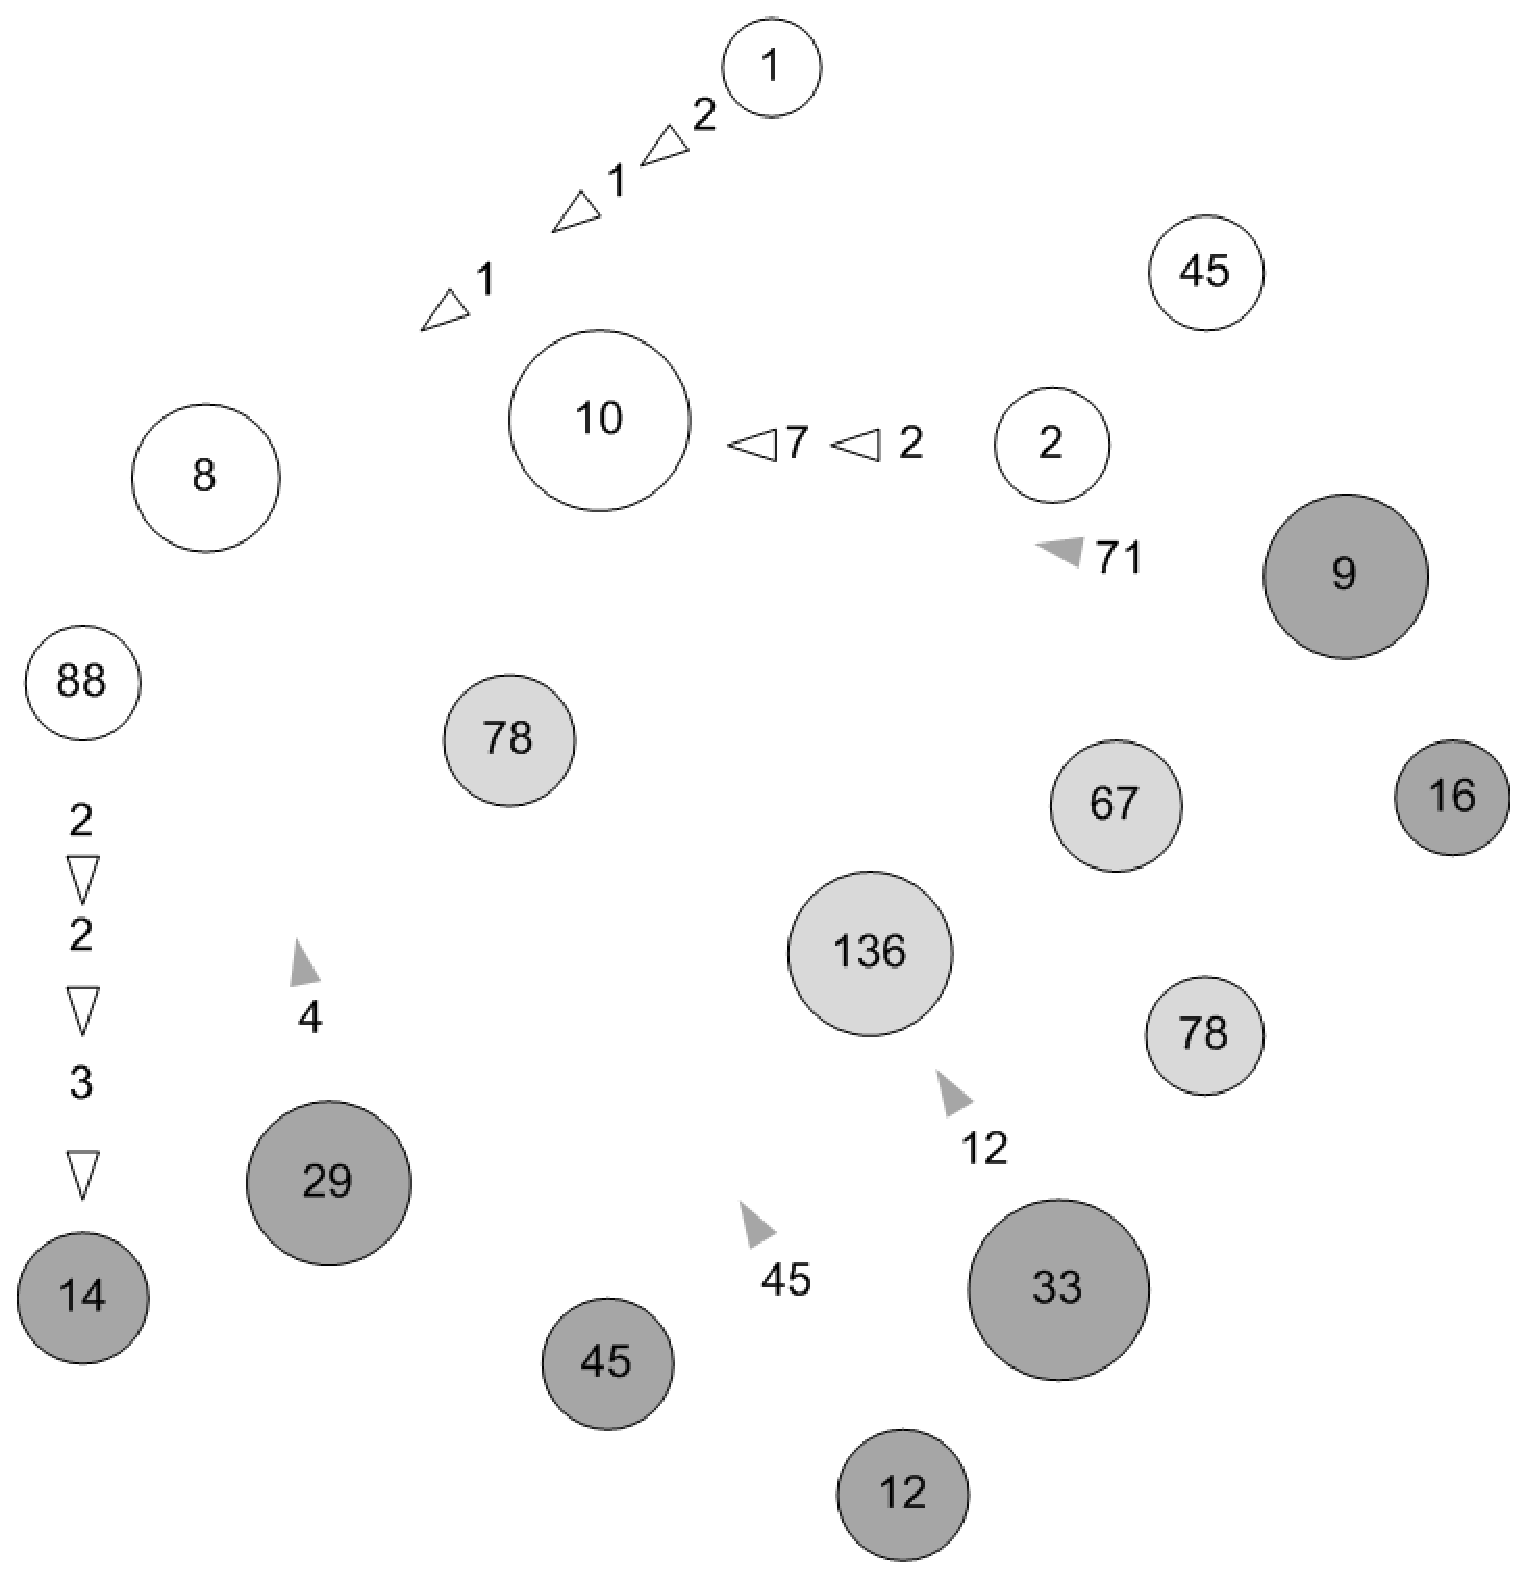
\epsfig{file=./imags/naves.eps,width=4cm}
\end{center}
\caption{Simulated screen shot of an early stage of a run in Planet Wars. White planets belong to the player (blue colour in the game), dark grey belong to the opponent (red in the game), and light grey planets belong to no player. The triangles are fleets, and the numbers (in planets and triangles) represent the ships. The planet size means growth rate of the amount of ships in it (the bigger, the higher).}
\label{figura:PlanetWars1}
\end{figure}

A Planet Wars match takes place on a map (see Fig. \ref{figura:PlanetWars1}) that contains several planets (neutral, enemies or owned), each one of them with a number assigned to it that represents the quantity of ships that the planet is currently hosting. 

The aim of the game is to defeat all the ships in the opponent's planets. Although Planet Wars is a RTS game, this implementation has transformed it into a turn-based game, in which each player has a maximum number of turns to accomplish the objective. At the end of the match, the winner is the player that remains alive, or that which owns more ships if more than one survives. 

There are two strong constraints which determine the possible methods to apply to design
a bot: a simulated turn takes \textit{just one second}, and the bot is \textit{not allowed to store any kind of information} about its former actions, about the opponent's actions or about the state of the game (i.e., the game's map).

Therefore, the aim in this paper is to study the improvement of a bot according to the state of the map in each simulated turn (input), returning a set of actions to perform in order to fight the enemy, conquering its resources, and, ultimately, wining the game. In the original game, only two bots are faced but in this paper it is studied what happen when we simulate 4 on 4 battles, i.e., when 4 bots are fighting in the same map.

%%%%%%%%%%%%%%%%%%%%%%%%%%%%%%%   SURVIVAL BOT  %%%%%%%%%%%%%%%%%%%%%%%%%%%%%%%%
%
\section{Survival Bots}
\label{sec:survival_bots}


A shape of co-evolution. They compete but the whole population (offspring) is improved.

Approaches:

% ------------------------------------------------------------------
%
\subsection{Steady-State Survival}
\label{subsec:steady-state}


% ------------------------------------------------------------------
%
\subsection{Generational Survival}
\label{subsec:generational}


%%%%%%%%%%%%%%%%%%%%%%%%%%%%%%%   EXPERIMENTS  %%%%%%%%%%%%%%%%%%%%%%%%%%%%%%%%
%
\section{Experiments and Results}
\label{sec:experiments}

Several experiments have been conducted in order to study different issues of the proposed approaches, but having in mind that the main objective is the improvement of bots using a co-evolutionary algorithm. The set of parameters considered in the GAs is shown in Table \ref{tabla:GA}. 
For each one of the presented approaches (combinations of fitness functions and knowledge-related methods), ten executions of the Co-GA have been performed.

\begin{table*}
\centering
\begin{tabular}{|c | c | c | c | c | c |}
\hline
Population Size & Generations & Crossover prob. & Mutation prob. & Elitism & Tournament size \\
\hline
100 & 200 & 0.6 & 0.1 & 20 & 2 \\
\hline
\end{tabular}
\caption{Table with the parameters used in the GAs.}
\label{tabla:GA}
\end{table*}


%%%%%%%%%%%%%%%%%%%%%%%%%%%%%%  CONCLUSIONS  %%%%%%%%%%%%%%%%%%%%%%%%%%%%%%%
%
\section{Conclusions and Future Work}
\label{sec:conclusions}

Several conclusions...


%ACKNOWLEDGMENTS are optional
\section{Acknowledgments}
%This paper has been funded in part by European and National projects FP7-318508 (MUSES) and TIN2011-28627-C04-02 (ANYSELF) respectively, project P08-TIC-03903 (EV\-ORQ) awarded by the Andalusian Regional Government, and project 83 (CANUBE) awarded by the CEI-BioTIC UGR.

%
% The following two commands are all you need in the
% initial runs of your .tex file to
% produce the bibliography for the citations in your paper.
\bibliographystyle{abbrv}
\bibliography{genebot} 

\end{document}
